\documentclass[11pt,a4paper, margin=1in]{article}
\usepackage{fullpage}
\usepackage{amsfonts, amsmath, pifont}
\usepackage{amsthm}
\usepackage{graphicx}
\usepackage{float}

\usepackage{tkz-euclide}
\usepackage{tikz}
\usepackage{pgfplots}
\pgfplotsset{compat=1.13}

\usepackage{geometry}
 \geometry{
 a4paper,
 total={210mm,297mm},
 left=10mm,
 right=10mm,
 top=10mm,
 bottom=20mm,
 }

 \author{
  Karaçanta, Kaan\\
  \texttt{e244854@metu.edu.tr}
}

\newcommand{\mySin}[1]{\textstyle\sin\left(#1\right)}
\newcommand{\myCos}[1]{\textstyle\cos\left(#1\right)}
\usepackage{hyperref}

\usepackage{inconsolata}
\usepackage{listings}
\usepackage{xcolor}
\usepackage[utf8]{inputenc}
\usepackage[T1]{fontenc}

\definecolor{codegreen}{rgb}{0,0.6,0}
\definecolor{codegray}{rgb}{0.5,0.5,0.5}
\definecolor{codepurple}{rgb}{0.58,0,0.82}
\definecolor{backcolour}{rgb}{0.95,0.95,0.92}

\lstdefinestyle{mystyle}{
    backgroundcolor=\color{backcolour},
    commentstyle=\color{codegreen},
    keywordstyle=\color{magenta},
    numberstyle=\tiny\color{codegray},
    stringstyle=\color{codepurple},
    basicstyle=\ttfamily\footnotesize,
    breakatwhitespace=false,
    breaklines=true,
    captionpos=b,
    keepspaces=true,
    numbers=left,
    numbersep=5pt,
    showspaces=false,
    showstringspaces=false,
    showtabs=false,
    tabsize=2
}

\lstset{style=myStyle}

\title{CENG 371 - Scientific Computing \\
Fall' 2024 - 2025 \\
Homework 2}

\date{}

\begin{document}
\maketitle

\noindent\rule{19cm}{1.2pt}

\section*{Question 2}

\begin{enumerate}

    \item \textbf{Comparison of Algorithms in Terms of Speed and Accuracy:}
    
    The plots of the runtime and relative error of Sherman's, Pickett's, and Crout's algorithms are shown in Figures \ref{fig:runtime} and \ref{fig:relative_error}, respectively. The runtime plot demonstrates the scalability of each algorithm with matrix size, while the relative error plot shows the accuracy of each method compared to the built-in LU decomposition. The following observations can be made from the plots:

    \begin{figure}[H]
        \centering
        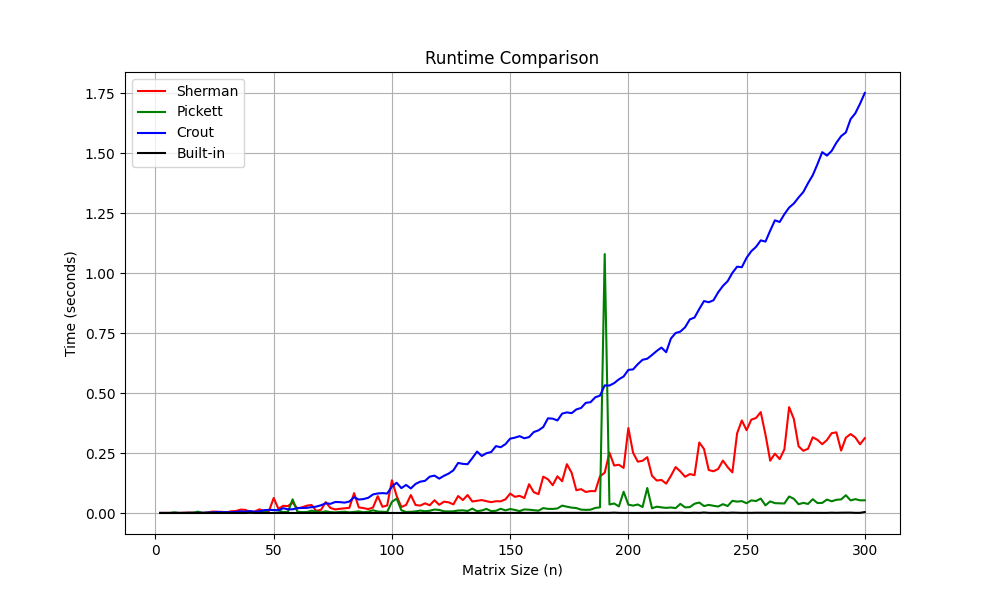
\includegraphics[width=1\textwidth]{runtime_comparison.png}
        \caption{Runtime Comparison of Sherman's, Pickett's, and Crout's Algorithms}
        \label{fig:runtime}
    \end{figure}

    \begin{figure}[H]
        \centering
        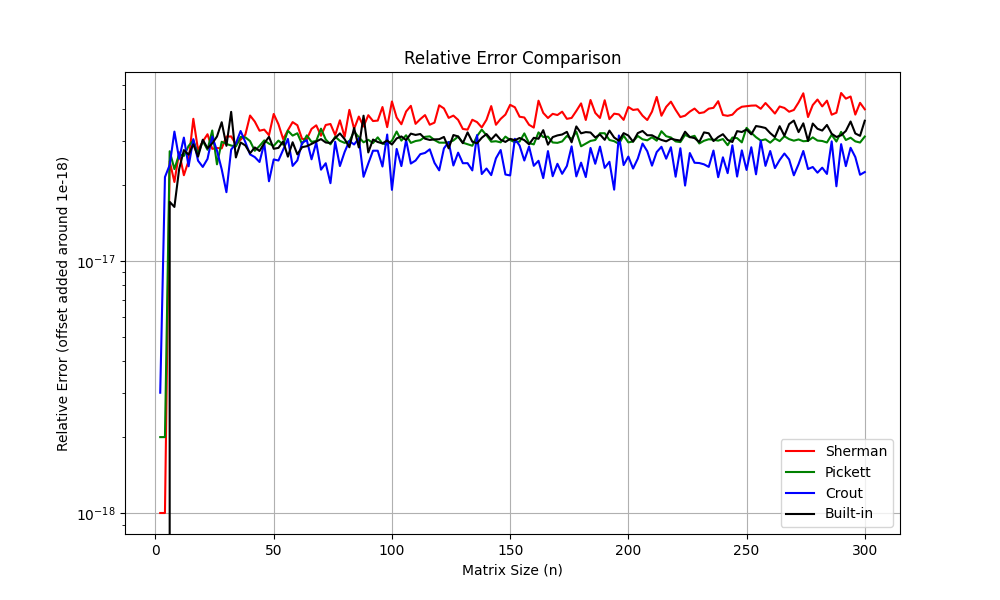
\includegraphics[width=1\textwidth]{error_comparison.png}
        \caption{Relative Error Comparison of Sherman's, Pickett's, and Crout's Algorithms}
        \label{fig:relative_error}
    \end{figure}
    
    The algorithms were compared based on runtime and relative error while factorizing Hilbert matrices of size \( n \) (from 1 to 300). The following findings were observed:
    
    \begin{itemize}
        \item \textbf{Sherman's Algorithm:} 
        Sherman's method demonstrates a consistent runtime that scales, a kind of, linearly with matrix size, making it competitive for larger matrices. Its accuracy is slightly worse compared to Pickett's and Crout's algorithms, possibly due to the small perturbation \( 1e{-12} \) added to the diagonal to avoid singularity, which may lead to cumulative numerical instability in the recursive steps. However, these errors are minimal, in a level almost equal to the machine epsilon and built-in LU decomposition, so it is negligible in my opinion.
        
        \item \textbf{Pickett's Algorithm:} 
        Pickett's method performs efficiently for smaller matrices but exhibits sharp runtime spikes for certain matrix sizes. These spikes might be caused by computational resources, operating system's scheduling etc. Despite these spikes, on average, Pickett's relative error is the closest across all methods to the built-in LU method, suggesting that it handles numerical stability well. Plus, for the big matrices as well, its runtime is the closest to the built-in LU method.

        \item \textbf{Crout's Algorithm:} 
        Crout's algorithm performs poorly in terms of runtime, significantly worse than Sherman's and Pickett's methods. This inefficiency increases as matrix size grows, making Crout's method the slowest of all. However, it maintains relative errors comparable to the other methods, indicating that it remains numerically stable, it produces even smaller relative errors than built-in LU decomposition for almost all matrix sizes.
        
        \item \textbf{Built-in LU:} 
        The scipy built-in LU decomposition function serves as a robust baseline. It outperforms all three algorithms in terms of runtime, as expected, and maintains a consistent relative error among all matrix sizes, although Crout's algorithm produces even smaller, it is negligible as these numbers are very close to the machine epsilon.
    \end{itemize}
    
    \newpage

    \item \textbf{Explanation of Observed Behavior:}
    
    \begin{itemize}
        \item \textbf{Runtime Spikes in Pickett's Algorithm:}
        The spikes in Pickett's runtime occur because the Schur complement computation occasionally involves ill-conditioned intermediate matrices. These numerical instabilities increase the computational effort required to solve linear systems during the recursion. These types of spikes can be solved by running the algorithm multiple times and taking the average runtime, but as it is a time consuming process and it does not happen that frequently, it is clearly an exception, I did not think that it is that important.

        \item \textbf{Crout's Poor Performance:}
        Crout's algorithm performs the worst in terms of runtime, might be due to its implementation. Unlike Sherman's and Pickett's methods, Crout's approach did not effectively calculate the results, this can be a result of the algorithm itself as well. However, it maintains a consistent relative error, even lower than the built-in as I explained before, so it can be a good alternative if the sizes are small. Plus, it gives a predictible runtime result as the size of the matrix increases.

        \item \textbf{Relative Error Analysis:}
        All algorithms maintain relative errors around \( 10^{-17} \), which corresponds to the limits of double-precision floating-point arithmetic. The differences in relative error are minimal, with Crout's method slightly outperforming Sherman's and Pickett's methods for larger matrices. This indicates that Crout's method handles numerical stability more effectively despite its higher runtime.

        \item \textbf{General Observations:}
        All algorithms show negligible relative errors. Probably the algoritmic designs of these methods are well enough to handle the numerical stability issues. As can be seen in Crout's algorithm's results, there can be trade-offs between runtime and accuracy, so it is important to choose the right algorithm based on the requirements of the problem. Moreover, some of the algorithms may show better or worse performances on specific architectures, or hardware, but as I have tested on my machine all of these, I can only say that these are the results I have obtained.
    \end{itemize}

    \textbf{Conclusion:} 
    \begin{itemize}
        \item \textbf{Crout's algorithm} Slightly better numerical stability and predictable behavior but slower runtime.
        \item \textbf{Pickett's algorithm} Flexible for structured matrices, but susceptible to runtime spikes, probably others are as well, but I only observed on this one.
        \item \textbf{Sherman's algorithm} Balanced performance with consistent runtime and error behavior.
    \end{itemize}

\end{enumerate}


\end{document}